\section{Suggested system} \label{app:sug_sys}
\subsection{System overview}
The system in mind requires three variable inputs:
\begin{enumerate}
\item The dump file obtained after running Frog with all NE's per item
\item The original data file with the documents (because the source isn't included in the dump file)
\item The search query
\end{enumerate}
A user of the system has two options: either acquire the NE's in a selected document (without necessary prior knowledge of its contents), or find a document that is most relevant to the search query of the user. The query has to be of the following format: $$TYPE{\text{:}}NE(+TYPE{\text{:}}NE)^n$$ An NE can be negated by putting a '!' right before the term. The result of running the code below using the default parameters can be seen in figure \ref{fig:sys_out}.

\subsubsection{Alternating the search query}\label{app:alt_query}
If the company \textit{Coca-Cola} is not classified as ORG, but as a MISC instead, the following search query will not retrieve results: $$ORG\text{:}Coca\text{-}Cola$$
However, adding another possible type to the query fixes the issue:
$$ORG\text{:}Coca\text{-}Cola\text{+}MISC\text{:}Coca\text{-}Cola$$
In contrast, when \textit{Coca-Cola} is not \emph{recalled}, there is no alternate query that will retrieve the NE. 

\begin{figure}
    \centering
    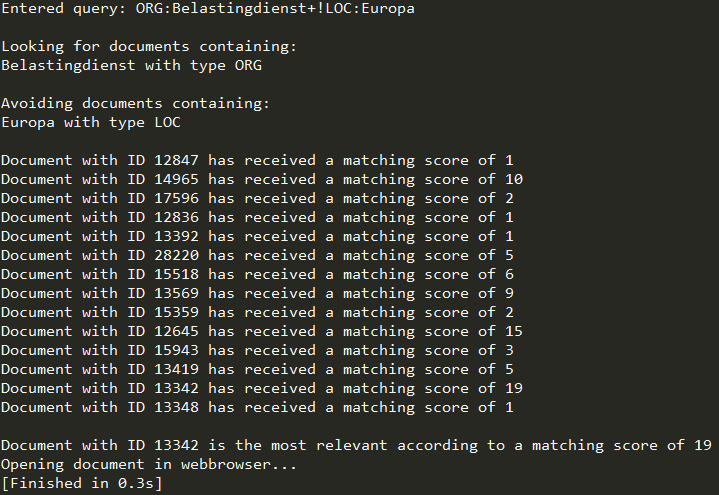
\includegraphics[scale=0.8]{fig/sys_out}
    \caption{The command line output running the code of the suggested system}
    \label{fig:sys_out}
\end{figure}

\subsection{Raw code}
\begin{lstlisting}
import json, re, webbrowser, sys, argparse
from operator import itemgetter

def main(dump_path, docs_path, query):
    with open(dump_path) as f:
        dump = json.load(f)

    winning_id = get_document(query, dump)

    with open(docs_path) as g:
        for doc in g:
            doc = json.loads(doc)
            if winning_id == doc['_id']:
                print 'Opening document in webbrowser...'
                webbrowser.open(doc['_source']['url'])    

def get_document(query, dump):
    """
    Opens the document most relevant
    to the query in your webbrowser from its 
    original source.
    """
    relevant_docs = []
    positive = []
    negative = []
    elements = query.split('+')

    print 'Entered query:', query

    ## Seperate the query into a list of wanted and unwanted entities in a doc
    for e in elements:
        entity_type, entity = e.split(':')
        if entity_type[0] == '!':
            negative.append((re.sub('!', '', entity_type), entity))
        else:
            positive.append((entity_type, entity))

    print '\n', 'Looking for documents containing:'
    for entry in positive:
        print entry[1], 'with type', entry[0]

    print '\n', 'Avoiding documents containing:'
    for entry in negative:
        print entry[1], 'with type', entry[0]

    for doc_id in dump:
        if matches_query(dump[doc_id], positive, negative):
            relevant_docs.append(doc_id)

    return most_relevant_doc_id(relevant_docs, query, dump)

def matches_query(doc, positive, negative):
    """
    Returns if the document matches the query
    by checking wanted and unwanted entities
    """
    match = False

    ## Look for a positive match
    for entity_type, entity in positive:
        if entity in doc['entities']:
            for tag in doc['entities'][entity]:
                t = tag.split('-')[1]
                if t == entity_type:
                    match = True
    
    ## If positive, look for a negative match
    if match:
        for entity_type, entity in negative:
            if entity in doc['entities']:
                for tag in doc['entities'][entity]:
                    t = tag.split('-')[1]
                    if t == entity_type:
                        match = False

    return match


def most_relevant_doc_id(relevant_docs, query, dump):
    """
    Returns the document ID with the highest
    matching score.
    """
    matching_scores = []
    for doc in relevant_docs:
        score = calculate_matching_score(dump[doc], query)
        matching_scores.append((doc, score))

    print ''
    for pair in matching_scores:
        print 'Document with ID %d has received a matching score of %d'%(int(pair[0]), pair[1])


    ID, best_score = max(matching_scores, key=itemgetter(1))
    print '\n', 'Document with ID %d is the most relevant according to a matching score of %d'%(int(ID), int(best_score)) 

    return ID
        

def calculate_matching_score(doc, query):
    """
    Returns the document's matching score
    to the query
    """ 
    elements = query.split('+')
    positive = []
    score = 0

    ## Get all wanted entities and their type out of the query
    for e in elements:
        entity_type, entity = e.split(':')
        if not entity_type[0] == '!':
            positive.append((entity_type, entity))

    ## Look for a positive match, and increase matching score accordingly
    for entity_type, entity in positive:
        if entity in doc['entities']:
            for tag in doc['entities'][entity]:
                t = tag.split('-')[1]
                if t == entity_type:
                    score += doc['entities'][entity][tag]

    return score

if __name__ == '__main__':

    p = argparse.ArgumentParser()
    p.add_argument('-dump', type=str, help='path to the dump with extracted entities per doc', default='data/lobby/dump')
    p.add_argument('-docs', type=str, help='path to original unprocessed documents', default='data/lobby/train_documents')
    p.add_argument('-query', type=str, help='Query used to find the desired document', default='ORG:Belastingdienst+!LOC:Europa')
    args = p.parse_args(sys.argv[1:])

    main(args.dump, args.docs, args.query)



 
\end{lstlisting}